\section{Project-Based Comparison}\label{sec:proj_eval}

The current projects for developing software in MANETs fall into three broad categories: runtimes, languages, and middleware, which offer increasing levels of abstraction for the developer. They can also be combined: a middleware solution can be written in a language which uses one of the basic runtimes for mobile devices. In many cases projects also provide additional resources for software development such as debuggers and emulators for testing code. Table\ref{table:projs} summarizes the representative projects discussed in this section with respect to the requirements in Section \ref{sec:manetrecs}. Broader overviews focusing only on middleware for MANETs can be found in~\cite{middlewaresurvey} and \cite{newmiddlewaresurvey}.

\begin{table*}\footnotesize
\centering
\caption{Projects Summary}
\begin{tabular}{|p{2.2cm}|p{2cm}|p{2.75cm}|p{2.7cm}|p{2.7cm}|} \hline
\textbf{Project} & \textbf{Category} & \textbf{Disconnection Handling} & \textbf{Addressing and Discovery} & \textbf{Communication} \\ \hline
LIME & Middleware & Tuple removal & Merged tuple spaces & Tuple space \\ \hline
MESHMdl & Middleware & Tuple removal & Tuple exchange & Tuple space \\ \hline
TOTA & Middleware & Connectionless & Tuple propagation & Tuple space \\ \hline
STEAM & Middleware  & Connectionless & Event content & Publish/subscribe \\ \hline
SyD & Middleware &  Object proxies &  Object type & Message passing \\ \hline
M2MI & Language & Connectionless &  Object type & Message passing \\ \hline
AmbientTalk & Language &  Flexible references &  Object type & Message passing \\ \hline
\begin{comment}YCab & Middleware &  State recovery &  Sessions, handles & Message passing \\ \hline\end{comment}
SpatialViews & Language & Connectionless & Object type & Code migration \\ \hline
.NET CF & Runtime &  None & URL & Sockets \\ \hline
Java ME & Runtime & None & URL & Sockets \\ \hline
\end{tabular}
\label{table:projs}
\end{table*}

\subsection{Project Overview}

\subsubsection{Runtimes}

Runtimes in this context are virtual machines for languages which are specifically intended for use on small, resource-constrained mobile devices. Runtimes are useful because they provide good portability for applications and thereby simplify some of the application development process.

Two common runtimes for mobile devices are Java ME~\cite{javame} and the .NET Compact Framework~\cite{dotnetcf}. A third runtime, BREW~\cite{brew}, is a proprietary product from Qualcomm. These runtimes focus on using few resources and providing libraries for application development, especially user interfaces. They do not provide much networking support beyond basic sockets and HTTP support. While it is possible to use these runtimes as foundations for better abstractions, they provide little on their own to support MANET applications and will not be considered in the following comparisons.

\subsubsection{Languages}

A language in this dissertation refers to any language, language extension, or library which provides new language constructs for programming in a MANET. Languages often include their own runtime or are built on top of existing runtimes. Libraries and language extensions are likely to be easier for developers to use if they are already familiar with the base language.

M2MI~\cite{m2mi}, AmbientTalk~\cite{ambienttalk}, and SpatialViews~\cite{nisv} are three language-based projects intended for MANETs. Many-to-Many Invocation (M2MI) avoids costly ad hoc routing and discovery by broadcasting messages. Messages are addressed by object type, so if a device hosts an object of the addressed type, it will pass the message to that object.

The advantage of M2MI is simplicity. As messages are simply broadcast without expectation of reply, there is no need to worry about return values or blocking while waiting for confirmation. At the language level, there is no difference on the sender's side between a message which is actually received and one which is not received by anyone. Though this provides simplicity, it also means more work for the programmer. As there is no guarantee of message delivery, any functionality beyond simple unidirectional message passing must be implemented on top of M2MI.

AmbientTalk is a complete object oriented language inspired in part by M2MI's message passing. AmbientTalk implements a higher level abstraction of resource discovery and disconnection handling which is absent from M2MI, but retains the idea of object handles and remote method invocations. All remote events are handled asynchronously by AmbientTalk through the registration of callbacks. A block of code may be registered to be invoked when discovering a certain resource type. AmbientTalk also adds the ability to receive values from method invocations on remote objects through the use of futures. By default, messages sent to remote objects are buffered until they can be sent. The programmer can also choose to break the connection and recall buffered messages.

SpatialViews takes a completely different approach than M2MI and AmbientTalk. SpatialViews is a language extension to Java ME which allows programs to iterate over groups of devices. The code inside the loop is executed on the initial device and then migrates to the next, eventually making its way back to the initial node. This allows for complex operations to be written easily, as the language has built-in support for such things actions as reduction operations. The iteration itself is generally done according to some physical layout, although it is possible to iterate over all objects or to use logical locations instead.

\subsubsection{Middleware}

Middleware is software which manages interaction and communication between applications, as well as providing various services which may be used by applications. Middleware may also include supporting libraries which can be used by applications.

LIME (Linda in mobile environment)~\cite{lime} is a well-established implementation of tuple spaces\cite{linda} for mobile environments. Each device or agent has its own tuple space, which can merge with remote tuple spaces when they come into range of each other. Tuples can be read and written from specific locations, but can also be read or written to the ``federated" tuple space which includes the local tuple space and any tuple spaces which are currently merged with it. However, the tuple will reside in a particular tuple space, so when that device or agent moves away, the tuples in that tuple space will move with it and be out of reach. LIME does not currently have an implementation intended for mobile devices smaller than laptops, though there are variations of LIME intended for sensors.

MESH\textit{Mdl}~\cite{meshmdl} is another tuple space implementation, but varies slightly from the LIME model. In MeshMdl, there is a single tuple space shared between all applications on a device. All communication between applications is done through this shared tuple space. Remote tuple spaces are not shared like in LIME, but are accessible for reads and writes only: it is not possible to remove tuples from a remote tuple space. MESH\textit{Mdl} supports mobile agents and recommends using them if actions need to be performed on a remote tuple space. MESH\textit{Mdl} also adds the idea of being able to automatically write, read, or block tuples from other tuple spaces.

Tuples on the Air (TOTA)~\cite{tota} also implements a tuple space for MANETs, but differs from LIME and MESH\textit{Mdl}. Rather than storing tuples on a particular device, tuples in TOTA are propagated through the network according to rules specified per tuple. As the tuples move through the network, they can acquire context information about the network, such as how many hops they have traveled from the source.

Haggle \cite{haggle} is a middleware for mobile networks which allows tagged data to persist in a publicly searchable storage space. The Haggle middleware focuses heavily on abstracting the network layers by implementing its own routing and naming schemes, which allows a single name to map to several addresses such as MAC addresses, phone numbers, or email. Haggle proposes folding in many routing protocols, MAC protocols, and application protocols into the middleware and dynamically selecting and combining them.

SyD (System on Mobile Devices)~\cite{syd} is a complete middleware solution for MANETs. The middleware centers around the idea of object registries which allows service registration and lookup. Methods can then be invoked on these remote objects. Disconnection is handled by allowing objects to also provide proxy objects. If an object is unavailable, the method invocation will be handled by the proxy object, which can then perform an action specific to that service. For example, the proxy may buffer the request and send it later, or send back a cached or default response.

STEAM (Scalable Timed Events and Mobility)~\cite{steam} is an event-driven middleware which uses a publish/subscribe\cite{psfaces} mechanism for propagating events. STEAM uses the concept of proximity groups for communication, limiting events to the local geographic area. Events are propagated by subscribers only when the subject and proximity match. Events are further filtered on the subscriber side by content, which determines if an event is delivered to the local application.

\subsection{Suitability for MANETs}

\subsubsection{Disconnection Handling}

The main challenge in MANETs is handling disconnections, which may be intermittent, prolonged, or permanent. For example, at a busy conference there may be many mobile devices in contact with each other, but distance and physical obstacles may cause intermittent disconnections. Routes may also break and reform due to mobility or channel variations, possibly causing prolonged disconnections, but connections are eventually regained. When the attendees all leave, it becomes unlikely their devices will ever be in contact with each other again, making the disconnection permanent. A programming environment for MANETs must be able to handle all three kinds of disconnections.

One solution, used in LIME, MESH\textit{Mdl}, and TOTA, is to use tuple spaces for communication. Tuple spaces exhibit both spatial and temporal decoupling, meaning that messages being sent do not need to be addressed to a particular recipient nor does the recipient need to be present when the message is sent. Tuple spaces generally operate by reading, writing, and taking tuples to and from a shared location. Rather than sending a message directly to a recipient, a tuple is written to the tuple space and can be read or taken from the tuple space by other clients. This allows the tuple space to withstand disconnections.

For example, a tuple may be written out to the tuple space and then retrieved by a different client an arbitrary amount of time later. The client which retrieves the tuple may not even be in existence when the tuple was written. However, there is still a problem if the writer of the tuple disconnects before the tuple is read by a receiver. For LIME and MESH\textit{Mdl}, where the tuple space is associated with a particular devices, the tuple space is only available when the sender and the receiver are able to communicate directly with each other. In TOTA, tuples are disseminated throughout the network and can survive even if the original sender disconnects.

A different approach, used by M2MI and STEAM, is to forgo connections completely. Messages in M2MI are sent with no expectation of reply. In the general case, messages are sent to a particular object type, to be processed by any device hosting an object of that type. Messages are broadcast with no buffering whether or not there is a receiver available. This provides even more decoupling than tuple spaces, but tuple spaces have the advantage of having some feedback about a tuple's status. The sender can check if a tuple has been removed from the tuple space or not. If it has, the sender can have some assurance the tuple was received by someone, otherwise it will be available until removed by the original sender or another client.

STEAM avoids connections by filtering events on the subscriber's side. This eliminates the need for publishers to keep track of subscribers and completely decouples the two. However, publish/subscribe in a MANET environment does not provide any message reliability. Any message reliability or disconnection feedback would need to be implemented on top of the publish/subscribe framework.

Code migration, the approach used by SpatialViews, does not maintain connections, but can be affected by disconnections if the device currently executing the mobile code fails or leaves the network before completion.  Most of the devices in the network will not be involved in executing code at any particular moment, in which case their failure or disconnection from the network would not have an effect. When it does have an effect, however, it may cause the entire iteration to fail. This can be mitigated by using a form of parallel iteration over the devices. Since the iteration order in SpatialViews is nondeterministic, it does not provide message reliability.

A third approach, implemented in AmbientTalk, relies on event handling and futures. Event handlers can be registered for various events, such as discovery of a service or disconnection of a remote object. Figure~\ref{fig:atpd} illustrates the use of two of these callbacks to discover a printer service. Once a printer is discovered, a document is sent to be printed and a status message is returned.  If a remote object is discovered and later moves out of range, AmbientTalk can call the disconnection code. By default, messages sent to a disconnected remote object will be buffered until it is possible to send them. This provides a solution for intermittent and even prolonged disconnections. If a remote object is disconnected for too long, the programmer can recall all buffered messages and close the connection.

\begin{lstlisting}[caption={Printer Discovery in AmbientTalk}, label={fig:atpd}]
 def print(doc) {
  when: Printer discovered: { |printer|
    when: (printer<-print(doc)) becomes: {|res|
      system.println("Status: " + res);
    };
  };
 };
\end{lstlisting}

AmbientTalk also offers AmbientReferences\cite{ambientrefs}, which are related to the M2MI model of object handles.  AmbientReferences have a specified flexibility which determines how disconnections are handled. Sturdy is the default model of using buffered messages which will be delivered upon reconnection. Elastic references wait a specified amount of time before severing the connection and rebinding to another object of the same type. Fragile references will break immediately upon disconnection and rebind to another object as quickly as possible.

The approach used by SyD is to offer the ability for the application designer to specify how to handle disconnections. In SyD, it is possible to provide proxy objects which will be called when the actual remote object is unavailable. These objects can then handle the invocation in an object-specific manner, such as buffering or returning a default value. \begin{comment}YCab provides an interface for storing application-specific data and restoring the state of the application upon reconnection to a given session.\end{comment}

\subsubsection{Addressing and Discovery}

Unlike a wired network with a fixed infrastructure, MANETs cannot depend on centralized look up services like DNS to find peers. Since devices are constantly joining and leaving the network and it is not possible to maintain IP addresses or URLs to locate resources, applications must be able to locate them dynamically.

The tuple space implementations of LIME, MESH\textit{Mdl}, and TOTA automatically discover neighboring tuple spaces. LIME will merge tuple spaces with the same name, while MESH\textit{Mdl} does not merge tuple spaces, but uses special tuples to provide a method of addressing a remote tuple space. Tuple spaces can be used for service discovery by writing out tuples which describe available services, or by writing out tuples intended for a specific service, which will read the tuples when it is available.

Addressing is not necessary in general in tuple spaces, as it can be assumed a given service and a client will have pre-agreed upon tuple template to use for communication. For example, a ubiquitous application used by a museum might have ``information points'' with information specific to a location. The information point does not need to even be aware of clients, nor do clients need to know any identifying information about the information point, as they will simply read available tuples from the information point's tuple space.

Object types for discovery and addressing is used by M2MI, AmbientTalk, and SpatialViews. This is based on the assumption that objects with the same name will implement the same services. M2MI and AmbientTalk use this with object handles which refer to a specific object type. When methods are invoked on a given handle, the remote object will correspond to the type of the object handle. M2MI, however, does not provide a method for discovery beyond manually sending out messages periodically and waiting for replies. AmbientTalk offers event handlers to be automatically called when objects of a specific type are discovered. These can be called exactly once or each time one is discovered.

SpatialViews uses object types along with spacial properties to define a ``view" of the network. Once a view is created containing a given object type, SpatialViews provides a method of iterating over the available nodes within that view. The code within the iterator is executed locally on the remote devices. After the code is run, the device locates another nearby node hosting an object of the correct type and the code migrates there. Within the iteration, the code can synchronously invoke methods on the local service through an object handle. In Figure~\ref{fig:svsm}, a simple SpatialView is created to broadcast a message in a chat application. The code within the \texttt{visiteach} block (line 4) is executed locally. Therefore, unlike the AmbientTalk printer example, \texttt{c.receive(...)} is a local method call, not a remote call.

\begin{lstlisting}[caption={Simple Messaging in SpatialViews}, label={fig:svsm}]
 spatialview v = ChatService;

 visiteach c : v {
   c.receive(sender, message);
 }
\end{lstlisting}

SyD also uses objects to invoke remote services, but it requires that these objects register themselves with neighboring devices, as well as locally. \begin{comment}YCab is interesting in that it allows applications to detect nearby sessions, then suggest a handle for themselves. If the handle is unique in the session, the client is allowed to join, otherwise the client is rejected. \end{comment}

The publish/subscribe model used by STEAM relies on subscribers knowing ahead of time what subscriptions are interesting to them. The publishers do not need to explicitly know who is subscribed, as messages are simply broadcast. However, it is possible to periodically send out messages describing available subscriptions.

\subsubsection{Flexible Communication}

Basic communication between devices in a network is generally accomplished in a one-to-one unicast manner. However, in a MANET, group communication is also common, due to the broadcast nature of wireless networking and the limitations of bandwidth. Collaborative applications, networked games, and streaming media also benefit from group communication. Having both one-to-one and group communication available in the programming environment is necessary, though it may be possible to implement one with the other.

Tuple spaces lend themselves naturally to group communication. Tuples are written to shared storage space, which is globally accessible. Since tuples can be read without being removed from the tuple space, tuples are inherently one-to-many. One-to-one communication is not as directly supported by tuple space. However, tuples can be sent to a specific recipient by setting one of the fields in the tuple to an agreed-upon address. The specified recipient can look for tuples addressed to itself and take them from the tuple space.LIME, MESH\textit{Mdl}, and TOTA support this type of communication. 

M2MI and AmbientTalk support object references which can refer to all objects of a type, a selected subset of those objects, or a particular object. These handles directly correspond to broadcast, multicast, and unicast. Since AmbientTalk expects return values from messages, it is possible to receive multiple replies when sending a multicast or broadcast message, resulting in event handlers running multiple times or the return value being set more than once.

Communication in SpatialViews is done through code and variable migration. This makes it very simple to perform complex group operations such as reductions over several devices, but it makes one-to-one communication difficult. Figure~\ref{fig:svpd} shows how it is necessary to set a variable to ensure a document is only printed by a single printer. There is also no method to provide reliable message delivery, other than iterating until a prearranged flag is set.

\begin{lstlisting}[caption={Printer Discovery in SpatialViews}, label={fig:svpd}]
 Container result = new Container();
 spatialview v = Printer;
 visiteach p : v {
    if(result.isEmpty()) {
       String result = p.print(document);
	    if(result == "success")
	       result.addElement(p.getName());
    }
 }
\end{lstlisting}

Similarly, publish/subscribe naturally supports group communication, but attempting to send a message to a particular recipient is not directly supported by the middleware. Publish/subscribe is intended to be used in situations with a single sender and multiple receivers and does not adapt well to sending a message to a single receiver. To do so would require the sender and receiver using a predefined addressing, similar to setting an agreed-upon tuple value in tuple spaces. Successful message delivery in the publish/subscribe is less likely than in a tuple space, since messages are not persistent in the way that tuples are.

\begin{lstlisting}[caption={LIME: Print Job Reaction}, label={fig:lpj}]
 LimeTupleSpace lts = 
   new LimeTupleSpace();
 lts.setShared(true);
 ITuple printjob = 
   new Tuple().addFormal(PrintJob.class);
 UbiquitousReaction ur = 
   new UbiquitousReaction(printjob, 
     this, Reaction.ONCEPERTUPLE);
 lts.addWeakReaction(new Reaction[] {ur});
\end{lstlisting}

\subsection{Applications}

To better understand the effect of using different programming approaches when developing applications, two separate applications were written using AmbientTalk, LIME, and SpatialViews. These projects were selected because they represent very different approaches and had publicly available implementations. For each application, we discuss issues with disconnections, discovery, and communication.

\subsubsection{Printer Discovery}

The printer discovery application illustrates how the different projects can be used to approach the problem of resource discovery in a changing network. The client needs to locate a device offering a printer service. Next it sends the print job to a printer it has found, then waits for a reply. The printer processes the job and sends back a success or failure message.

Disconnection can occur at different points in this process. The printer may go out of range after the client has discovered it, but before the job is sent, or it may go out of range after the job is sent, but before the result is returned. In AmbientTalk, the default way of handling both cases is to wait until the printer can be contacted again and then resume the connection. The print job or result message will be buffered until the connection can be made again and then the message will be delivered. This works well in the case where there is only transient disconnection, but if a client has permanently left the area of the printer the application may wait forever unless the programmer explicitly uses a timeout.

In SpatialViews, the only way to communicate between nodes is to visit them in the course of an iteration over all nodes which offer a given service. With the SpatialViews implementation of printer discovery, disconnection after discovery and before sending back the success message are essentially the same. The iteration will never complete and the originating node will eventually timeout.

One of the strengths of tuple spaces is temporal decoupling. The sender and receiver do not both need to be present at the same time for a message to be sent. The LIME version of printer discovery does not face the disconnection issues above, partially because a print job remains in the tuple space until a result tuple is received. A printer which reads the print job and then goes out of range does not affect the operation. If the client is not in range when the result tuple is sent, but reconnects later, the result tuple will still be available for it to read. Even if the client permanently leaves an area, a different printer can pick up the print job instead. The downside of this approach is that multiple printers may process the same job, wasting resources.


In this example, addressing and discovery are needed to find a printer service and also to send the result message. AmbientTalk and SpatialViews handle addressing with interface types. The printer offers a service with a typed interface and the client is able to find nearby services of a given type. Discovery is also built into both AmbientTalk and SpatialViews. In AmbientTalk, a callback function is set up to be called when the printer service is discovered, as shown previously in Figure~\ref{fig:atpd}. SpatialViews uses the idea of an iterator which loops over objects of a certain type nearby. In this respect, AmbientTalk is more reactive, while SpatialViews is proactive. The disadvantage to the SpatialViews approach is the service must be available at the time of the iteration, otherwise it will complete without a result. It will then be up to the programmer to retry the iteration until it is successful.

Discovery in LIME merely requires the registration of reactions to tuple templates. Addressing the printer is not necessary, but the result message contains a print job identifier so the client knows which job it represents.

Printer discovery does not really involve group communication, but there is one-to-one communication in the sending of the print job and the result message. In AmbientTalk, an object handle to the remote printer service is created when the the printer is found. The print job is then sent by invoking a method on the handle and waiting for a return value. On the printer side, it only needs to return a value, it does not require any knowledge of the client.

For SpatialViews, care must be taken to make sure the print job only goes to a single printer. Since the only method of communication is to visit every printer available, it is necessary to set a flag in a shared variable indicating the print job was already successfully printed and subsequent printers do not need to address it, as seen in Figure~\ref{fig:svpd}. Again, the printer does not need to know anything about the client.

In LIME, all communication is also inherently group communication, so the result tuple needs to be explicitly addressed to the client using a some sort of identification. The client will be waiting for a tuple with that specific ID.

\subsubsection{Chat}

The second example is a chat application. Clients can send out public or private messages. Public messages are delivered to all other chat clients nearby, while private messages are directed to a specific recipient. As in most chat applications, there is no history and clients do not expect to receive messages sent earlier or when disconnected. Disconnection can occur at any time while clients are exchanging messages.

Disconnection has less effect in this application than with printer discovery, as the clients do not depend on the delivery of messages to continue operating. However, the AmbientTalk implementation does buffer both public and private messages and delivers them when the client reconnects, as this is built into the language. LIME also handles disconnection well in this case, since there is no need to guarantee message delivery. 

SpatialViews suffers from the same issue in the printer discovery example: if the code migrates to a section of the network which then becomes disconnected from the rest of the network, or the current node goes down, the iteration just stops. Since each message is a separate iteration, it will not affect the overall operation of the application.

Addressing is handled similarly to the printer discovery example, except the user needs to know the names of other users when sending private messages. The AmbientTalk version notifies the user when other clients come into range and adds their name and object handle to a list. Figure~\ref{fig:svchat} shows the implementation of the methods for sending out messages. Public messages are sent out to an AmbientReference, defined in line 1, which only needs to know the interface name and implicitly tracks individual clients.

\begin{lstlisting}[caption={Chat in SpatialViews}, label={fig:svchat}]
def all := ambient: Chatter 
    withCardinality: omni 
    withElasticity: fragile;

def sendAll(message) {
  all<-send(message, name);
};

def send(buddy, message) {
  def b := buddy_list.get(buddy);
  b<-send_private(message, name);
};
\end{lstlisting}

SpatialViews, like in the printer discovery application, iterates over all nodes with the chat interface, delivering the message to each as it visits. This is shown in Figure~\ref{fig:svchat}. For private messages, it still must iterate in the same manner, but the recipient is encoded in the message. Unfortunately, this means private messages still require visiting every node, possibly without even reaching the recipient in the case of disconnection. Likewise, LIME must rely on encoding the recipient in the message tuple and assuming no one but the intended client will read the message.

Group communication is natural for public messages and one-to-one communication for private messages. All three projects handle group communication well. AmbientTalk has omni-handles which refer to all interfaces of a given type and will broadcast the message to all nearby clients. The only communication in SpatialViews and LIME are essentially group communication, so for one-to-one communication, SpatialViews and LIME require the programmer to implement an addressing scheme on top of the group communication. The client side of the application needs to pick out private messages intended for it and ignore the rest.

\subsection{Experimental Results}

This section compares the performance of AmbientTalk, LIME, and SpatialViews in a regular wired LAN and in a MANET context using EXata.

The wired LAN environment provides a nearly ideal network in which the cost of communication is very low, there is little contention for the communication channel, all nodes are connected directly to each other, and collisions are minimal. By minimizing these factors, it is possible to focus the experiment results on the overhead of the programming environments. In these experiments, all nodes were directed connected to a 100Mb/s switch, providing essentially an independent, one hop channel for each pair of nodes

The results using EXata more accurately reflect the MANET environment. For these experiments, all communication was performed through EXata, which emulated an 802.11b ad hoc wireless network with an available bandwidth of 11Mb/s.

\begin{figure}
\centering
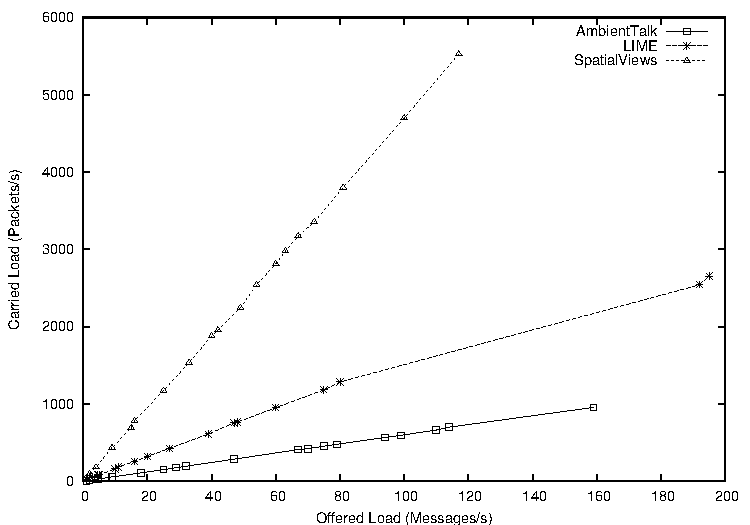
\includegraphics{figures/overhead-wired.pdf}
\caption{Communication Overhead with Wired Links}
\label{fig:overhead-wired}
\end{figure}

\begin{figure}
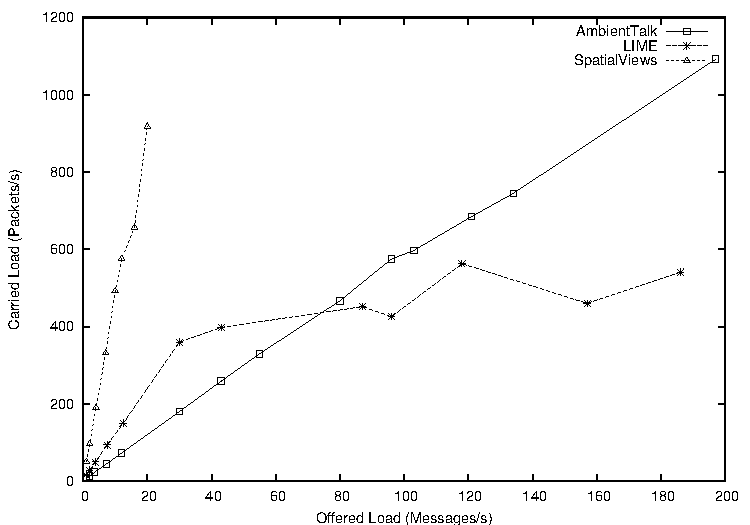
\includegraphics{figures/overhead-qualnet.pdf}
\caption{Communication Overhead with Simulated Wireless Links}
\label{fig:overhead-qualnet}
\end{figure}

\subsubsection{Communication Overhead}

AmbientTalk, LIME, and SpatialViews use very different messaging systems. This experiment demonstrates the overhead for each using a client-server setup as the simplest base case. Messages are sent out from the sever to the client at an increasing rate. The number of IP packets generated by doing so include control and discovery packets. Each node is within wireless range of the others so all communication is performed over single hop routes. Figure~\ref{fig:overhead-qualnet} and Figure~\ref{fig:overhead-wired} show the results from wired LAN and QualNet, respectively.

AmbientTalk has the lowest overhead, as it is simply performing a method call on a remote object and there is no return value. LIME requires some communication to alert merged tuple spaces of the messages' presence and then more communication to actually transfer the tuple. SpatialViews shows the highest amount of overhead, which is expected since it is migrating code and data to communicate a simple message. 

Although the results were similar in the wired LAN and EXata, the performance of SpatialViews was considerably slower, peaking at 20 msgs/s, while in the wired LAN it was possible to reach 117 msgs/s. This is due to contention for the wireless channel. It is also worth considering that LIME and AmbientTalk use asynchronous messages while SpatialViews uses a blocking synchronous message send. This allows LIME and AmbientTalk to take advantage of system level buffers, while SpatialViews cannot.

\begin{figure}
\centering
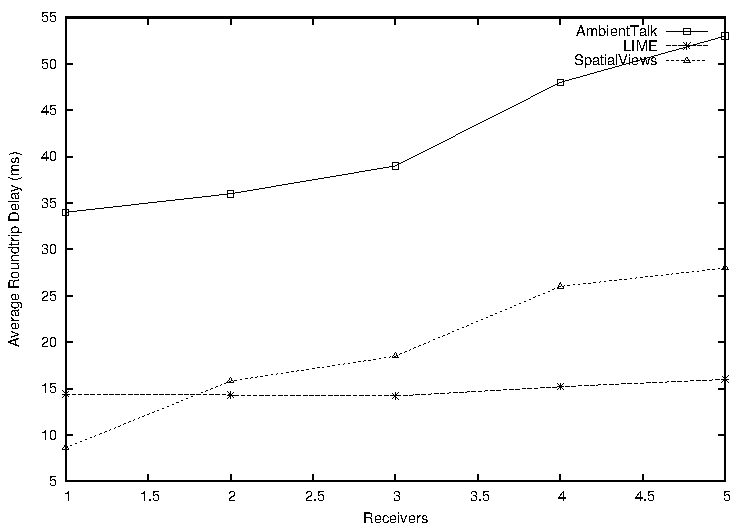
\includegraphics{figures/multicast-wired.pdf}
\caption{Group Communication with Wired Links}
\label{fig:multicast-wired}
\end{figure}

\begin{figure}
\centering
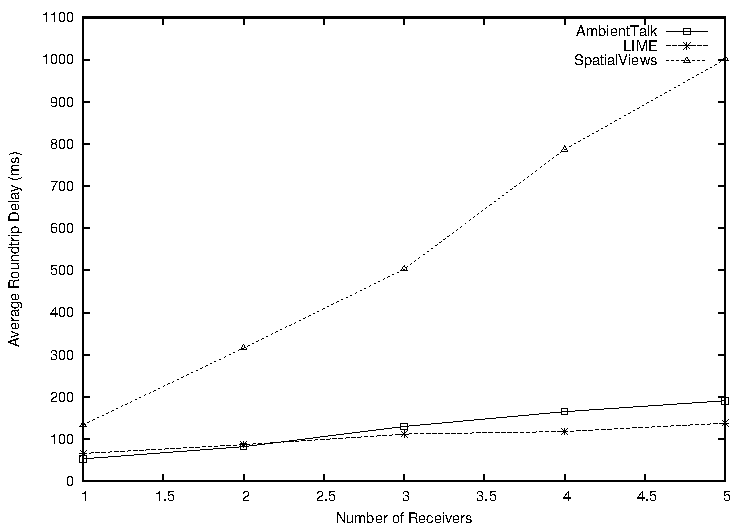
\includegraphics{figures/multicast-qualnet.pdf}
\caption{Group Communication with Simulated Wireless Links}
\label{fig:multicast-qualnet}
\end{figure}

\subsubsection{Group Communication}

In this experiment we consider the common situation where one node needs to request information from the rest of the network and then collect the results, with increasing numbers of receivers. The application sends out a message then measures the time elapsed for responses.  For SpatialViews, this involves visiting each node and that node then visiting the sending node. The AmbientTalk version uses an omnihandle, as in the chat application, to broadcast the handle of the sender and then the receivers use the handle to send a return message. For LIME, each message is sent as a tuple, to which the receivers send a response tuple. Again, the network is set up so that no node is farther than one hop from any other node. Figures~\ref{fig:multicast-qualnet} and ~\ref{fig:multicast-wired} show the results.

In the wired LAN, LIME shows the least variation as the number of receivers increases. This is because the sender writes out a single tuple and each receiver can respond independently and in parallel. SpatialViews slows down considerably as the number of receivers increases, since SpatialViews visits each receiver in turn and waits on a response before continuing. The delay for AmbientTalk is the highest but does not increase quite as quickly as SpatialViews. Although AmbientTalk uses a single send at the application level, messages to individual receivers are sent serially, causing the delay for the last receiver to be higher than the first. 

When run using EXata, the effect of using the wireless channel is seen again. The delay with AmbientTalk and LIME increases, but not as dramatically as SpatialViews, which reaches a delay of about 1 second with 5 receivers, while a single receiver averages 134 ms. As in the previous experiment, the traffic generated by SpatialViews quickly creates conflicts in the wireless channel, causing retransmission and delay at the MAC layer.

\subsubsection{Mobility and Disconnection}

\begin{figure}
\centering
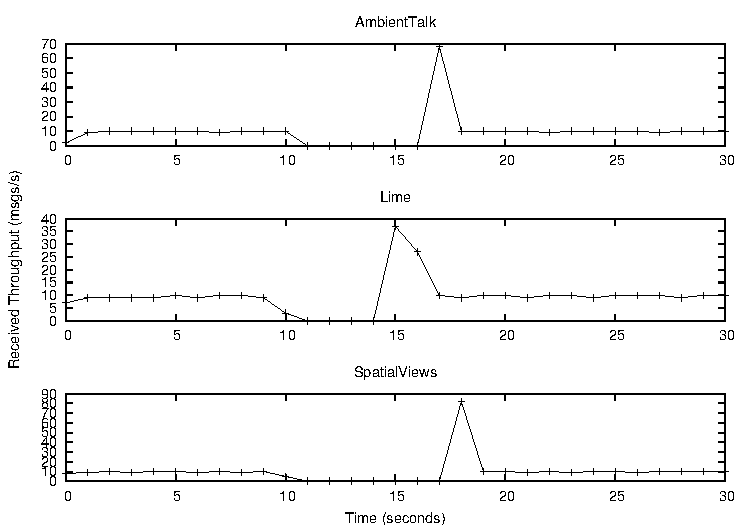
\includegraphics{figures/disconnection.pdf}
\caption{Disconnection Recovery}
\label{fig:disconnection}
\end{figure}

\begin{figure}
\centering
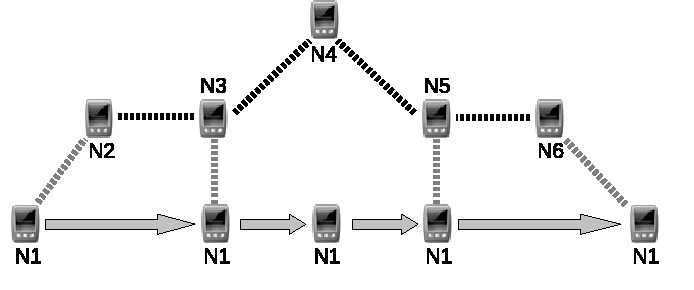
\includegraphics{figures/network.pdf}
\caption{Simulated Mobility Scenario}
\label{fig:network}
\end{figure}

\begin{figure}
\centering
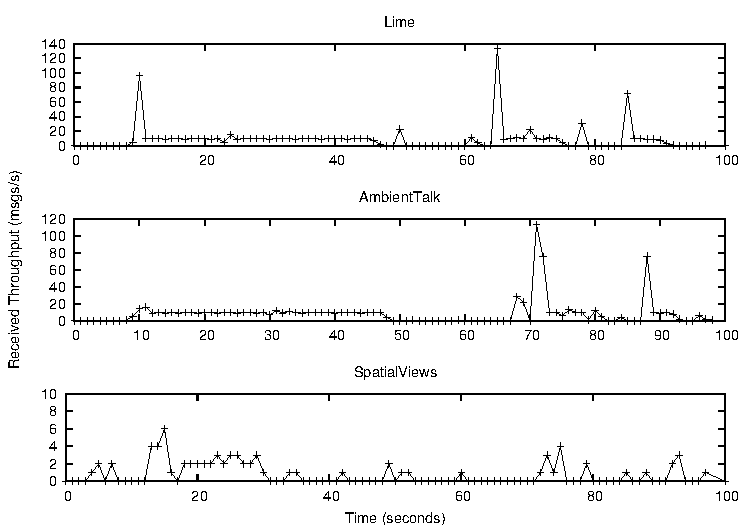
\includegraphics{figures/mobility-results.pdf}
\caption{Client-Server Throughput with Mobility}
\label{fig:mobility-results}
\end{figure}

In order to isolate and examine disconnection recovery, a simpler experiment in a wired LAN was performed, still using the same client-server application. In this case, a 5 second disconnection was caused by turning the network interface off and then turning it back on. Each project reacted similarly, as shown in Figure~\ref{fig:disconnection} though LIME showed the fastest recovery time. Interestingly, SpatialViews exhibited delivery of buffered messages. As SpatialViews does not buffer messages itself, this buffering was the result of the operating system attempting to locate the remote node.

Using EXata, it was possible to evaluate the projects in a mobile environment which provided disconnections, routing changes, and multi-hop communication. For this experiment, the network layout and mobility pattern shown in Figure~\ref{fig:network} was used. Node 1 user the same client-server application as in the first experiment and is attempting to send messages to Node 4. The distance between the two nodes forces a multi-hop route through the intermediate nodes. Node 1 moves from left to right at a constant rate during a time period of 100 seconds. This experiment again measures message delivery rate. Results are shown in Figure~\ref{fig:mobility-results}. 

The large spikes for the AmbientTalk and LIME results indicate the delivery of buffered messages. For AmbientTalk, the sender did not begin until the receiver was discovered, while LIME began sending messages immediately. The flat part of the graphs indicates when Node 1 was in between Node 3 and Node 5 and was outside the range of both. SpatialViews did not perform well in this experiment because it lacks the sophisticated disconnection handling and message buffering of the other two experiments. Also, the code migration was difficult, more time consuming, and more susceptible to disconnections. As in the previous experiments, this demonstrates the difference between experiments using a wired LAN compared to a simulated wireless network. 
